\documentclass[../ClassicThesis.tex]{subfiles}
\begin{document}

%************************************************
\chapter{Curves/Deus}\label{ch:curves}
%************************************************

\section{Cutting curved shapes}

Approximating curved shapes with parts created by the laser cutter is a special challenge because only 2d shapes can be cut. There are several approaches to make the cut material bendable, for example, paper can already be bent because of the material properties, acrylic if it is heated and wood with the help of living hinges.

Theoretically, this only enables the possibility to create shapes from developable surfaces (like cylinders) but no doubly curved ones (like spheres). Since our meshes are based on triangles, which are themselves 2D, our meshes are always developable.

\section{General approach}

In our implementation, we use bends as joint type as an alternative to, for example, finger joints. Therefore, it is based like the finger joint generation on the plate graph. It is separated into two important steps. First, our implementation analyses which parts bend. Second, it creates a flatted shape from the curved parts.
%The first one annotates each connection between plates if this should be a bending joint or not and the second creates a flatted shape from the plates that are connected with bends.

\section{Setting the joint type}

In this step, we try to find out which connections between two plates could be a bending joint so that the resulting shape of the connected plates is flattable without overlaps. An example for a model which surface is not devlopable without overlaps is shown in Figure \ref{fig:overlaps}.

\begin{figure}[h]
  \centering
  \begin{subfigure}[b]{0.49\textwidth}
    \centering
    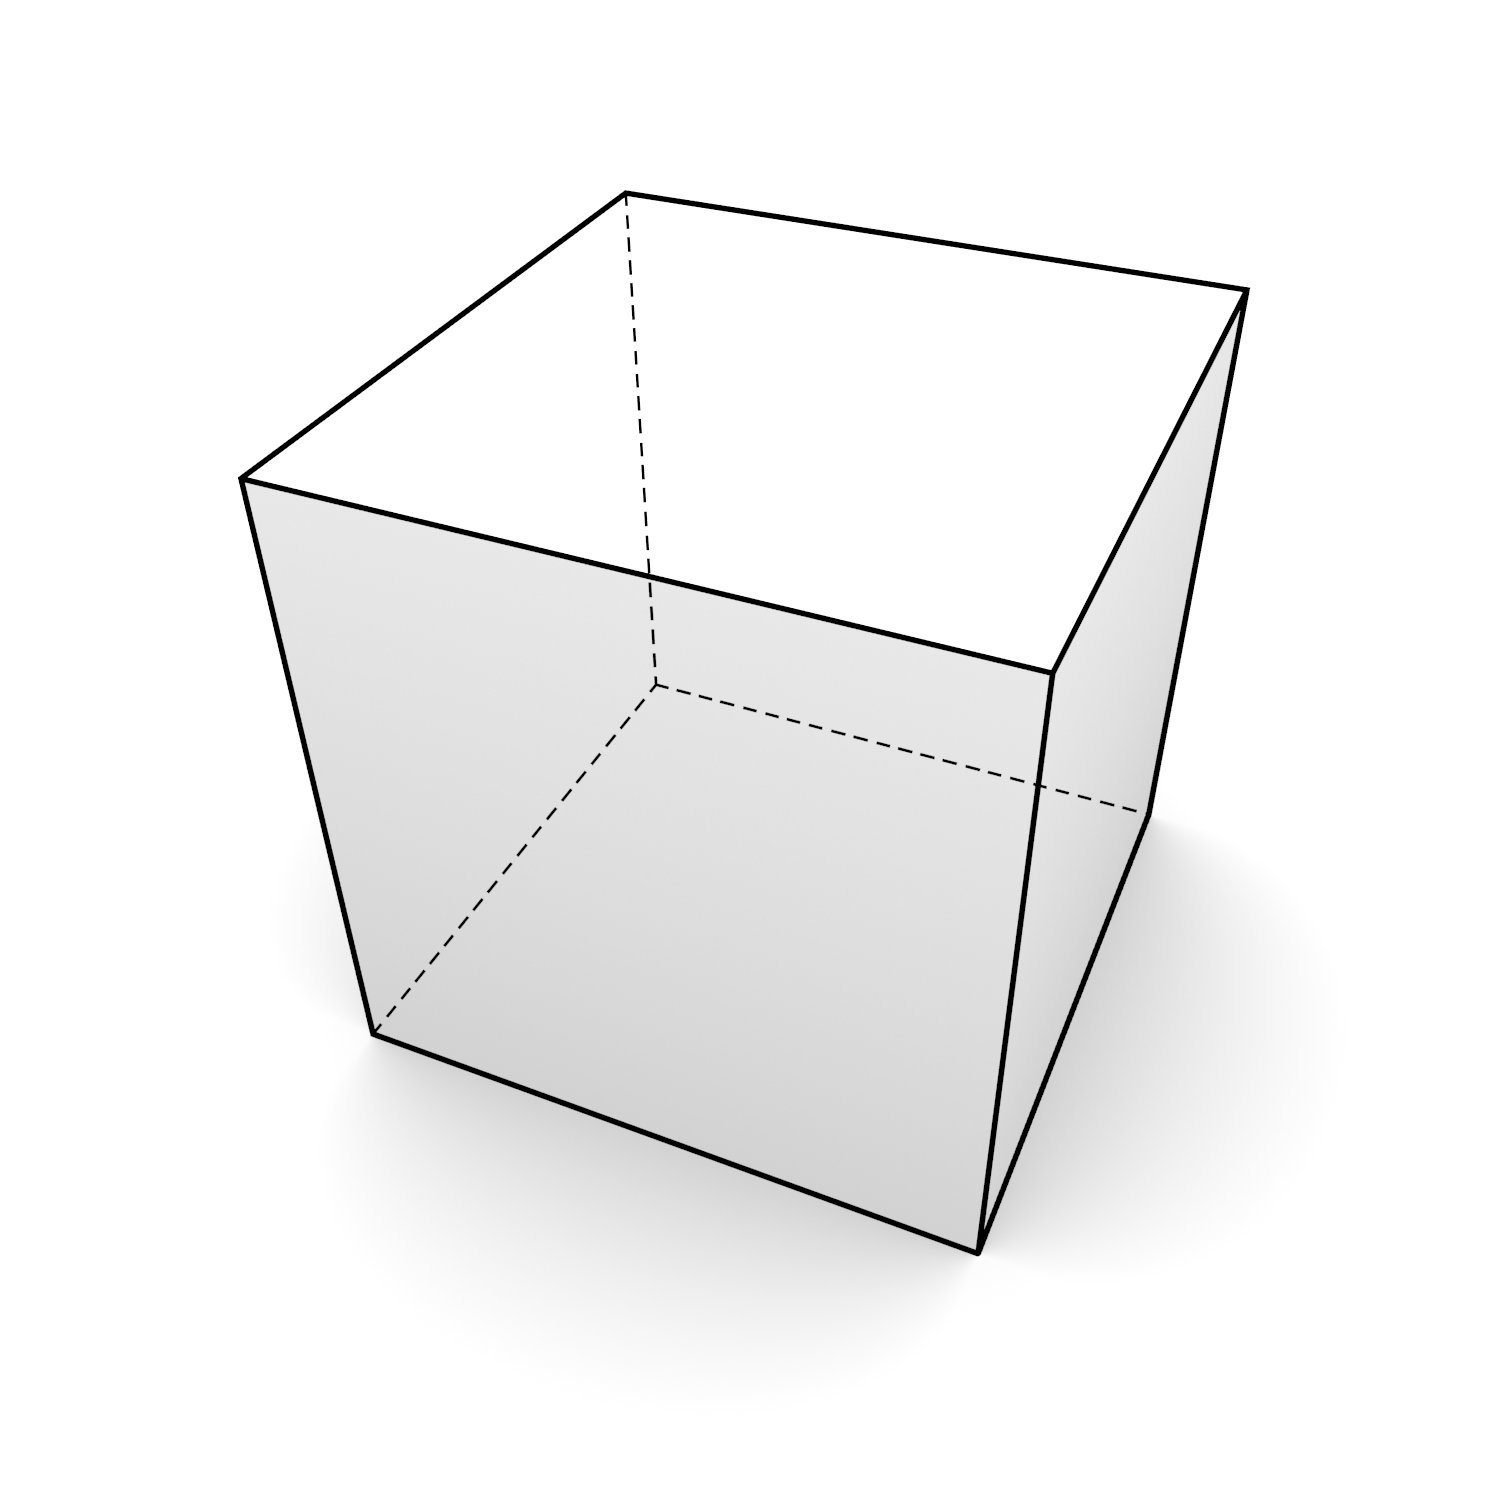
\includegraphics[width=\textwidth]{07-no_overlaps}
    \caption{A cubes surface can be developed without overlaps.}
    \label{fig:overlaps:no-3d}
  \end{subfigure}
  \begin{subfigure}[b]{0.49\textwidth}
    \centering
    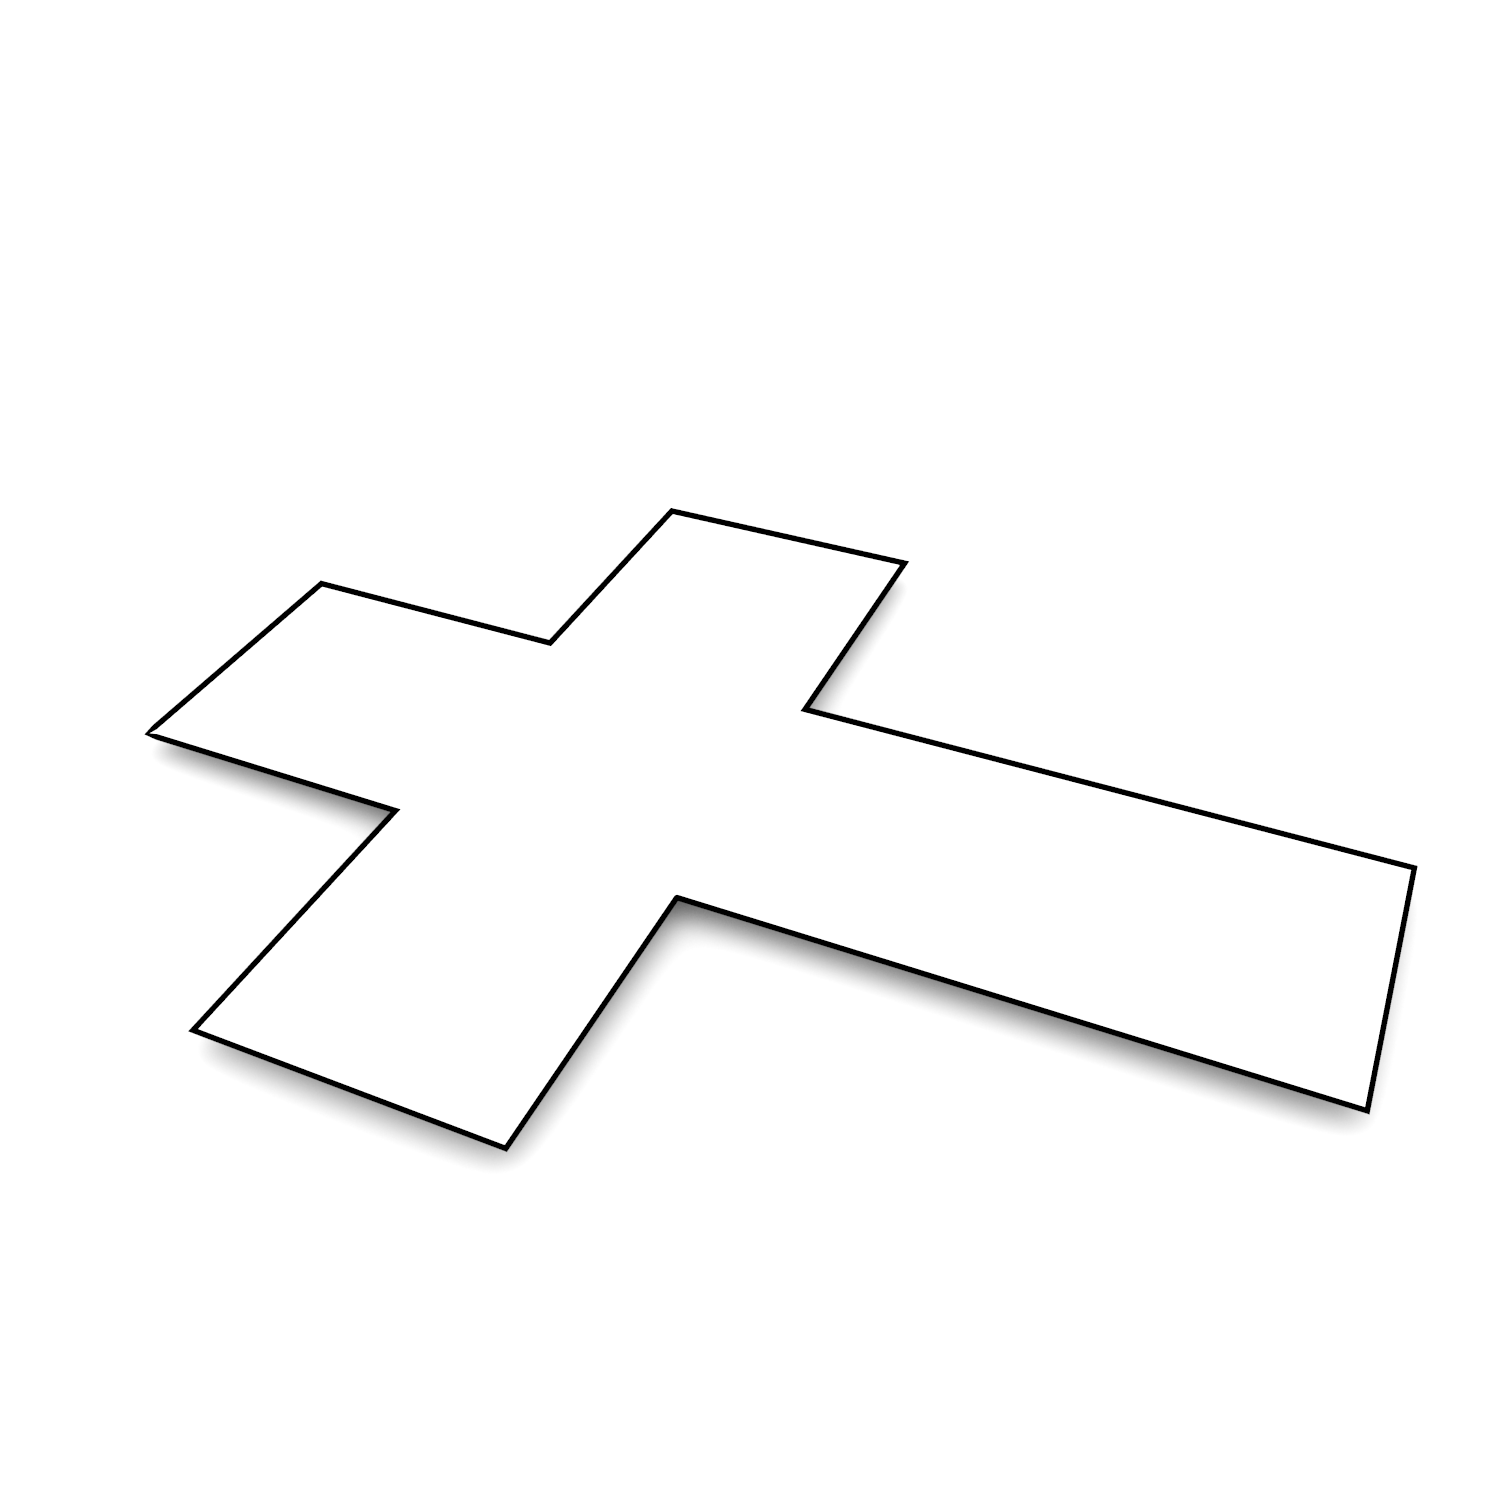
\includegraphics[width=1\textwidth]{07-no_overlaps_2d}
    \caption{One possible developed surface of a cube.}
    \label{fig:overlapsh:no-2d}
  \end{subfigure}
  \begin{subfigure}[b]{0.49\textwidth}
    \centering
    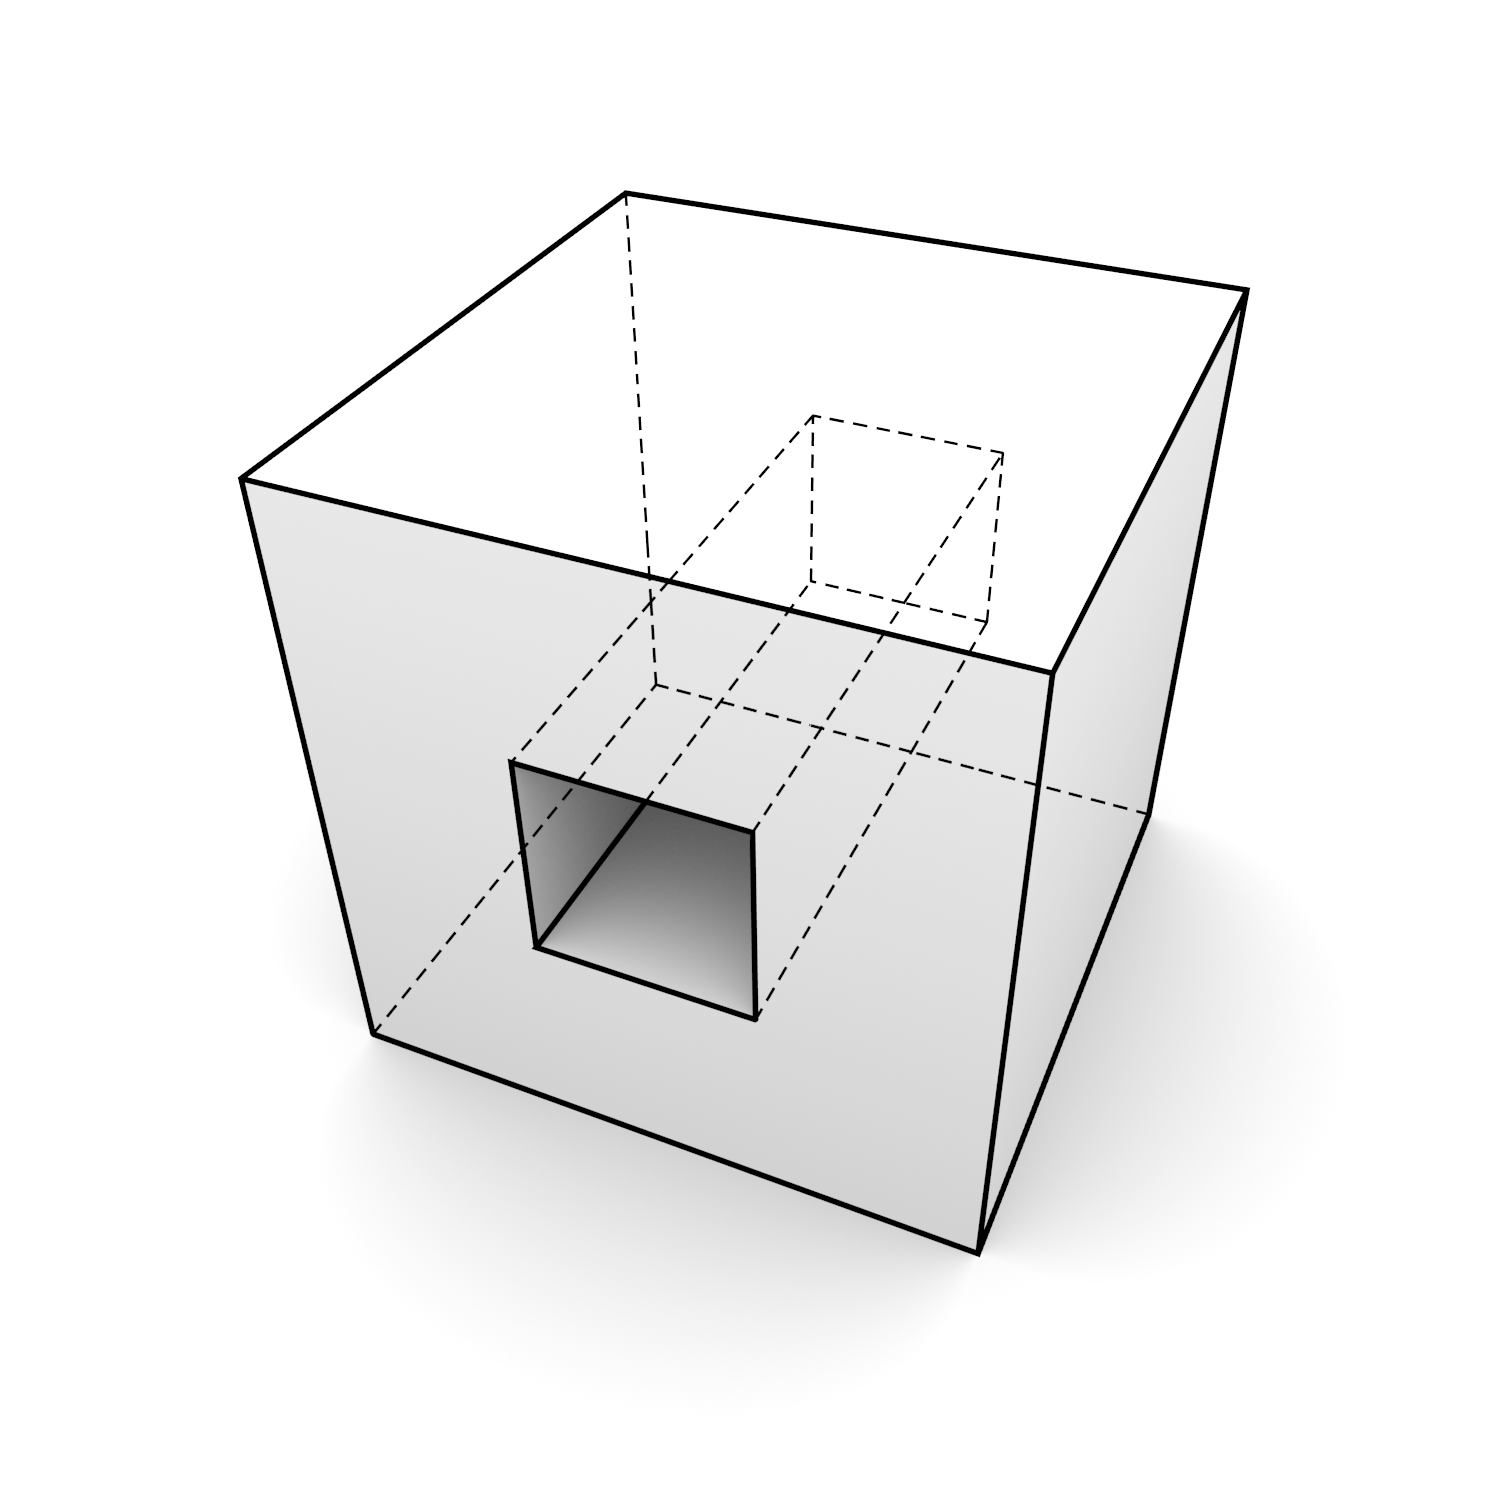
\includegraphics[width=\textwidth]{07-overlaps}
    \caption{The surface of an Cube with hole can not be developed without overlaps.}
    \label{fig:overlaps:some-3d}
  \end{subfigure}
  \begin{subfigure}[b]{0.49\textwidth}
    \centering
    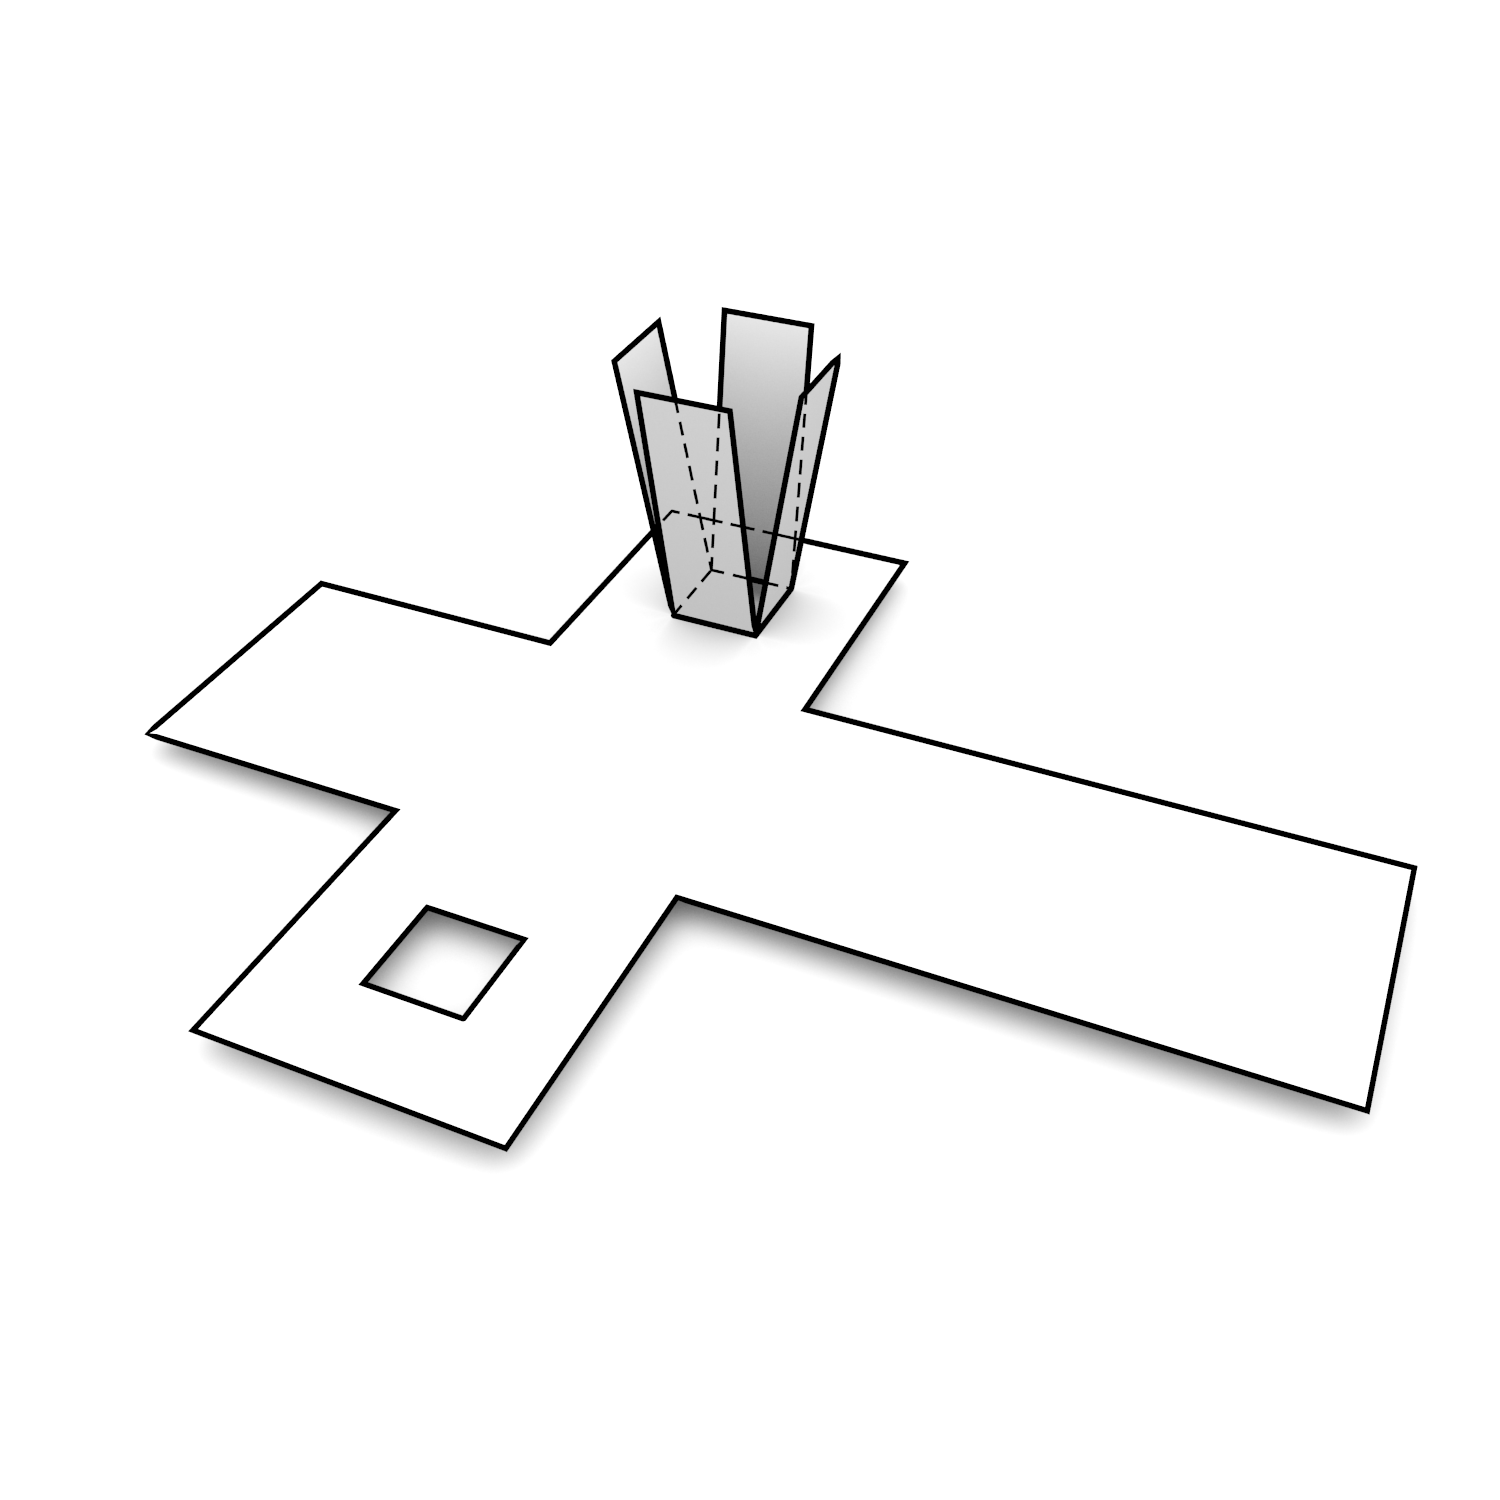
\includegraphics[width=1\textwidth]{07-overlaps_2d}
    \caption{The shapes inside the hole will always overlap some part of the developed surface.}
    \label{fig:overlaps:some-2d}
  \end{subfigure}
  \caption{A scene graph showing a box, composed of plates.}
  \label{fig:overlaps}
\end{figure}

To do so we start with one plate and check for all the connections it has:
\begin{itemize}
\item Is this connection not set already?
\item Is the connection angle near enough to 180\textdegree which means bending the material this far is possible? (What near enough means depends on the used material)
\item Is it possible to add the shape of the connected plate without overlapping the already existing shape?
\end{itemize}
If the answer is yes to all, the connected plate is added to this plate and they form a bent plate. This is repeated for all the connections of the bent plate until thy are all set to be a bending or a finger joint.
If after this some plates are not assigned to a bent plate the process is repeated for one of these until no one is left.

%shorten this sentence:
To check if a plate could be added to an existing bent plate we merge all the finger joint shapes of the outer connections of the bent plate and those of the probably added plate to the corresponding shape except for the ones that are from the connection between the bent plate and the new one. Then we calculate the intersection of this two. If the result is empty there are no overlaps, the plate can be safely added to the bent plate and the connection annotated as a bending joint.

If one of the conditions is not fulfilled the connection can't be a bend and is annotated as finger joint.

\section{Building the bent plates}
%TODO find subsection title
For building the bent plates our implementation starts with one plate of the plate graph and traverses the graph along the marked bend connections. This way all directly ore indirectly connected plates (via bend connections). Form these one bent plate is created. If there are plates in the plate graph that are covered by this process, it is repeated with one left plate until no plate is left.

\subsection{Traverse along bend connection}

While traversing along the bend connections the transformations matrices for the plates are calculated.

For the first plate the matrix is already known. It is the rotation matrix of its shape.

For the other plates it is important make sure that they keep in touch with the connected plate while laying them into the xy-plane. Therefore the bend angle must be calculated which is 180\textdegree  minus the angle between the connected plates (this angle is already known from the plate graph creation). Additionally the bend axis is determined building the cross product of the two normals of the connected plates. This way the axis does not only lay at the right place but also points in the right direction (which it would not it only the connection line between the two plates is used). The angle and the axis are used together to create the rotation matrix to lay the plate in the same plane like the previous plate. To get the final transformation matrix this must be multiplied by the transformation matrix of the previous plate.

\section{Alternative solutions}

\end{document}